\sectionframe{Szenarienmethode}
\begin{frame}
 \frametitle{Beispiel: Relieve Äthiopien}
 Langfristige Lagerhauskapazität: 8
 \begin{block}{Lagerhausbedarf:}\scriptsize
  \centering
  \begin{tabularx}{\textwidth}{l*{4}{>{\centering\arraybackslash}X}}
   \toprule
      &  Szenario I &  Szenario II &  Szenario III &  Szenario IV\\
     Ressource & (30\%) & (30\%) & (25\%) & (15\%)\\
   \midrule
    Nahrung 	& 4 & 2 & 3 & 4\\
    Trinkwasser & 3 & 5 & 3 & 5\\
    Medikamente & 3 & 3 & 1 & 4\\
   \bottomrule
  \end{tabularx}
 \end{block}
 \begin{block}{Kurzfristige Lagerhauskosten}
  \begin{itemize}
    \item 3500\$ für ein Nahrungsmittel-Lagerhaus
    \item 1600\$ für ein Trinkwasser-Lagerhaus
    \item 5200\$ für ein Lagerhaus für Medikamente
  \end{itemize}
 \end{block}
\end{frame}

\begin{frame}
 \frametitle{Zweistufige stochastische Optimierung}
 \begin{figure}
  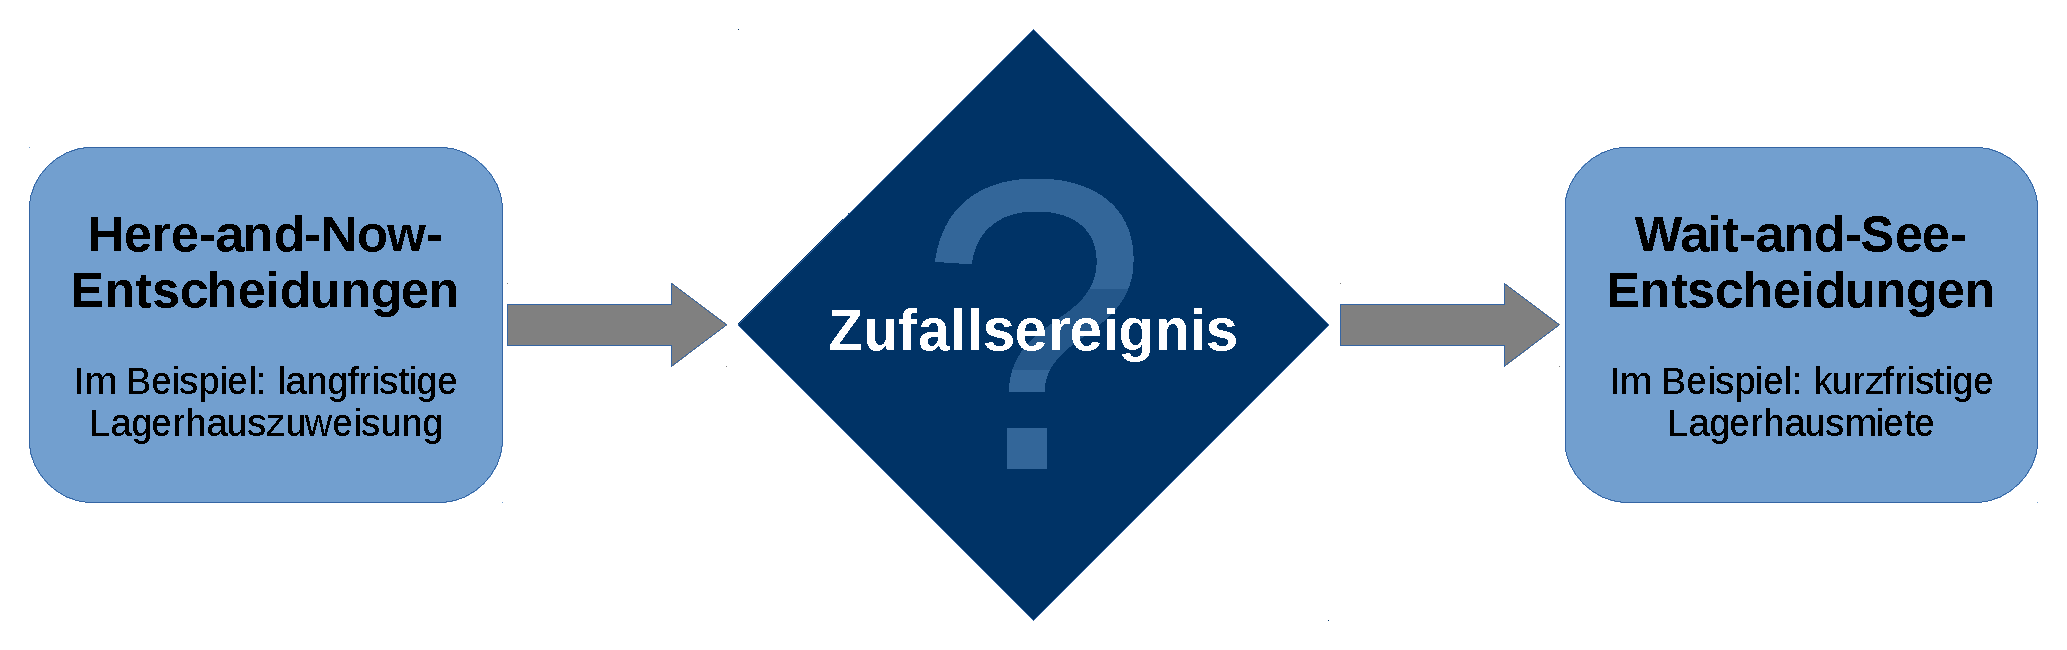
\includegraphics[width=\linewidth]{Bilder/Szenarienmethode}
 \end{figure}
 \begin{block}{Szenarienmethode}
  \begin{itemize}
   \item Spezialfall der zweistufigen stochastischen Optimierung
   \item Zufallsereignis = Eintritt eines von endlich vielen Szenarien
   \item stochastische Zielfunktion wird meist durch deren Erwartungswert ersetzt
  \end{itemize}
 \end{block}
\end{frame}

\begin{frame}
 \frametitle{Äquivalentes deterministisches Modell bei der Szenarienmethode}
 \begin{itemize}
  \item Indexmenge~$I$ der Szenarien
  \item Parameter~$p_i$: Eintrittswahrscheinlichkeit von Szenario~$i\in I$
  \item Szenariounbhängige Parameter und Here-and-Now-Entscheidungsvariablen haben keinen Szenarioindex
  \item Szenarioabhängige Paramter und Wait-and-See-Entscheidungsvariablen haben einen Szenarioindex
  \item Erwartungswert der Zielfunktion ist bei endlichen Szenarien eine Konvexkombination und damit linear
 \end{itemize}
\end{frame}

\begin{frame}
 \frametitle{Modell: Stochastische Ressourcenplanung}
 \footnotesize
 \begin{tabularx}{\linewidth}{lL}
  \multicolumn{2}{l}{\textbf{Indexmengen}:}\\
     $I$ & Menge der Szenarien\\
     $R$ & Menge der Ressourcen\\
  \multicolumn{2}{l}{\textbf{Parameter}:}\\
     $p_i$ & Eintrittswahrscheinlichkeit von Szenario~$i\in I$\\
     $c_r$ & Kosten für kurzfristige Zusatzkapaztität von Ressource~$r\in R$\\
     $d_{ri}$ & Bedarf an Ressource~$r\in R$ in Szenario~$i\in I$ \\
     $k$ & Zu verteilende Kapazität für langfristige geplante Ressourcen\\
  \multicolumn{2}{l}{\textbf{Entscheidungsvariablen}:}\\
     $x_{r}$ & Langfristig eingeplante Kapazität für Ressource~$r\in R$\\
     $y_{ri}$ & Kurzfristige angeschaffte Zusatzkapaztität für Ressource~$r\in R$ in Szenario~$i\in I$\\[1ex]
  \multicolumn{2}{l}{\textbf{Modellbeschreibung}:}\\[1ex]
  \multicolumn{2}{l}{
      $
      \begin{array}{rllr}
	\min & \multicolumn{3}{l}{
		  \displaystyle\sum_{i\in I}p_i\cdot\left(\sum_{r\in R}c_r\cdot y_{ri}\right)
		}\\[3ex]
	s.t. & \displaystyle\sum_{r\in R} x_{r} \leq k &  & \mathrm{(I)}\\
	      & x_r + y_{ri} \geq d_{ri}  & \quad\forall r\in R, i\in I  & \mathrm{(II)}\\[.8ex]
	      & x_r, y_{ri} \in \mathbb{Z}^+ & \quad\forall r\in R, i\in I &\\
      \end{array}
      $ 
  }\\[1ex]
 \end{tabularx}
\end{frame}



